\documentclass{report}

%Packages pour les langues
\usepackage[utf8]{inputenc}
\usepackage[T1]{fontenc}
\usepackage[french]{babel}
\usepackage{lmodern}
%Package pour la mise en forme (marges)
\usepackage[a4paper]{geometry}
\geometry{hscale=0.85,vscale=0.85,centering}
%Packages pour les formules de Maths
\usepackage{amsmath}
\usepackage{amssymb}
\usepackage{mathrsfs}
%Packages des images
\usepackage{graphicx}
\usepackage{subfigure}
\usepackage{wrapfig}
\usepackage{caption}
%\usepackage{subcaption}
\usepackage{float}
%Packages pour le glossaire
\usepackage{glossaries}
%\usepackage[xindy]{glossaries}
\makeglossaries
%Package pour colorier le code Matlab (copyright Jérémy Fauvel)
\usepackage{listings}
\usepackage[usenames,dvipsnames]{color}

%Code pour afficher du code Matlab
\definecolor{MyDarkGreen}{rgb}{0.0,0.4,0.0}
\lstset{language=Matlab, frame=none, basicstyle=\small\ttfamily, keywordstyle=[1]\color{Blue}\bfseries, keywordstyle=[2]\color{Purple}, keywordstyle=[3]\color{Blue}\underbar, identifierstyle=, commentstyle=\usefont{T1}{pcr}{m}{sl}\color{MyDarkGreen}\small, stringstyle=\color{Purple}, showstringspaces=false, tabsize=5, morekeywords={xlim,ylim,var,alpha,factorial,poissrnd,normpdf,normcdf}, morekeywords=[2]{on, off, interp}, morekeywords=[3]{FindESS, homework_example}, morecomment=[l][\color{Blue}]{...}, numbers=left, firstnumber=1, numberstyle=\tiny\color{Red}, stepnumber=1}





\begin{document}
\begin{titlepage}
\title{Rapport de stage - IRR \\ Implémentation et application d'un algorithme dynamique hybride pour le contrôle d'articulations flexibles}
\date{3 Mars 2014 - 31 Août 2014}
\author{Auteur: \bsc{Guedelha} Nuno \\ Tuteur: \bsc{Stasse} Olivier}
\end{titlepage}



\graphicspath{{illustrations/}}
\maketitle

%Rennomer la table des matières en Sommaire
\renewcommand{\contentsname}{Sommaire}
\tableofcontents
\listoffigures
\listoftables

%=============== Macros =================

%=============== variable fichier de figures ==============================

\newcommand{\myFiguresFile}{}
\newcommand{\setmyFiguresFile}[1]{\renewcommand{\myFiguresFile}{#1}}

%=============== include 1 figure =========================================

\ifx \incFig \undefined
\def \incFig [#1]#2{\includegraphics[width=#2, page=#1]{figs/\myFiguresFile}}
\fi

%=============== Display 1 figure =========================================

\ifx \dispFig \undefined
\def \dispFig [#1]#2#3#4#5%
{
\begin{figure}[#1]
  \begin{center}
  \includegraphics[width=#3, page=#2]{figs/\myFiguresFile}
  \IfStrEq{#4}{}{}{%
    \caption{#4}  % legende
    \label{#5}    % pour citer le numéro de figure
  }
  \end{center}
\end{figure}
}
\fi

%=============== 2 sous-figures alignées horizontalement =================

\ifx \dispTwoFig \undefined
\def \dispTwoFig [#1]#2#3#4#5#6#7%
{
\begin{figure}[#1]
\begin{center}
  \subfloat[#3 \label{#7.a}]{\includegraphics[width=7cm, page=#2]{figs/\myFiguresFile}}\hspace{1cm}
  \subfloat[#5 \label{#7.b}]{\includegraphics[width=7cm, page=#4]{figs/\myFiguresFile}}\hspace{1cm}
  \caption{#6}  % legende \\
  \label{#7} % pour citer le numéro de figure
\end{center}
\end{figure}
}
\fi

%=============== 3 sous-figures alignées horizontalement =================

\ifx \dispThreeFig \undefined
\def \dispThreeFig [#1]#2#3#4#5#6#7#8#9%
{
\begin{figure}[#1]
\begin{center}
  \subfloat[#3 \label{#9.a}]{\includegraphics[width=5cm, page=#2]{figs/\myFiguresFile}}\hspace{1cm}
  \subfloat[#5 \label{#9.b}]{\includegraphics[width=5cm, page=#4]{figs/\myFiguresFile}}\hspace{1cm}
  \subfloat[#7 \label{#9.c}]{\includegraphics[width=5cm, page=#6]{figs/\myFiguresFile}}\\
  \caption{#8}  % legende
  \label{#9}    % pour citer le numéro de figure
\end{center}
\end{figure}
}
\fi

%=============== 2 ou 3 colonnes alignée horizontalement ==================

\ifx \minipages \undefined
\def \minipages [#1]#2#3#4#5#6#7#8%
{
\begin{minipage}[#2]{#3\textwidth}
  #6
\end{minipage}
\begin{minipage}[#2]{#4\textwidth} \hfill
  #7
\end{minipage}
\IfStrEq{#1}{3}%
{
\begin{minipage}[#2]{#5\textwidth} \hfill
  #8
\end{minipage}
}
}
\fi

%=============== exemples ==================================================

%\begin{minipage}{.3\textwidth} \hfill
%  \begin{align*}
%  D_{O} = \lbrace &\textbf{d}_{Ox}, \textbf{d}_{Oy}, \textbf{d}_{Oy}, \\
%  &\textbf{d}_{x}, \textbf{d}_{y}, \textbf{d}_{z} \rbrace \subset M^{6}
%  \end{align*}
%\end{minipage}
%\begin{minipage}{.4\textwidth} \hfill
%  \begin{tabbing}
%  \= $\textbf{d}_{Ox}$ \= vecteur unitaire de rotation autour de $O_{x}$\\
%  \> $\textbf{d}_{Oy}$ \> vecteur unitaire de rotation autour de $O_{y}$\\
%  \> $\textbf{d}_{Oz}$ \> vecteur unitaire de rotation autour de $O_{z}$\\
%  \> $\textbf{d}_{x}$  \> vecteur unitaire de translation le long de $O_{x}$\\
%  \> $\textbf{d}_{y}$  \> vecteur unitaire de translation le long de $O_{y}$\\
%  \> $\textbf{d}_{z}$  \> vecteur unitaire de translation le long de $O_{z}$\\
%  \end{tabbing}
%\end{minipage}

%=============== autres macro textuelles ===================================

\newcommand{\cad}[0]{\textnormal{c'est à dire }}

\newcommand{\valTextwidth}[0]{\thetextwidth}

\newcommand{\valTextwidthUnit}[1]{\printinunitsof{#1}\prntlen{\textwidth}}

\newcommand{\valInUnit}[2]{\printinunitsof{#1}\prntlen{#2}}

%affichage des largeurs de zone texte
%\usepackage{layouts}
%\printinunitsof{cm}\prntlen{\textwidth}

\newcommand{\newglossdef}[3]
{\newglossaryentry{#1}%
{%
  name={#2},%
  description={#3}%
}}


%========================================

%%%%%%%%%%%%%%%%%%%%%%%%%%%%%%%%%%%%%%%%%%%%%%%%%%%%%%%%%
\chapter*{Remerciements}
\addcontentsline{toc}{chapter}{Remerciements}

Je voudrais remercier, avant tout, tous ceux qui ont rendu cette expérience possible, et très enrichissante.\\
Je tiens à remercier dans un premier temps, toute l’équipe pédagogique du Master I.R.R. et les intervenants professionnels responsables de la formation, pour avoir assuré la partie académique de celle-ci. Je remercie Mme. Viviane Cadenat et M. Michel Taix pour leurs conseils sur les critères de choix d'une formation de 2ème cycle en Robotique, qui ont facilité mon orientation à l'origine de mon inscription en Master I.R.R.\\
Je remercie également Monsieur Vincent Durola, mon tuteur pédagogique attitré, pour ses conseils concernant la mission de ce stage, conseils qui m'ont permis de prendre du recul par rapport à mes tâches et aux différents aspects techniques.\\
Je tiens à remercier tout particulièrement et à témoigner toute ma reconnaissance aux membres de l'équipe Gepetto, pour l’expérience enrichissante qu’elles m’ont permis de vivre durant ces six mois au sein du LAAS :\\
Monsieur Olivier Stasse, pour m’avoir intégré rapidement au sein du laboratoire et m’avoir accordé toute sa confiance ; pour le temps qu’elle m’a consacré tout au long de cette période, sachant répondre à toutes mes interrogations ; sans oublier sa participation au cheminement de ce rapport.\\
Monsieur Jean Paul Laumond, Maximilien Naveau, Justin Carpentier, ainsi que l’ensemble des membres de l'équipe Gepetto pour leur accueil sympathique et leur coopération professionnelle tout au long de ces six mois.\\
Tous ceux qui ont délivré des formations techniques sur la planification de mouvements, la dynamique inverse et les algorithmes de contrôle.\\

\vspace{0.3cm} % retour à la ligne


%%%%%%%%%%%%%%%%%%%%%%%%%%%%%%%%%%%%%%%%%%%%%%%%%%%%%%%%%

\newacronym{rneaLabel}{RNEA}{Recursive Newton-Euler Algorithm}
\newacronym{crbaLabel}{CRBA}{Composite Rigid Body Algorithm}
\newacronym{abaLabel}{ABA}{Articulated Body Algorithm}

\glsaddall
\printglossary

%%%%%%%%%%%%%%%%%%%%%%%%%%%%%%%%%%%%%%%%%%%%%%%%%%%%%%%%%

\chapter*{Introduction}
\addcontentsline{toc}{chapter}{Introduction}

\section*{contexte}


\section*{problème posé et objectifs}


\section*{étude bibliographique}


\section*{annonce du plan}



%%%%%%%%%%%%%%%%%%%%%%%%%%%%%%%%%%%%%%%%%%%%%%%%%%%%%%%%%
\chapter{Concepts généraux sur le contrôle dynamique des robots totalement actionnés}

\section{généralités sur le contrôle en couple ou position (vitesse ou accélération), et cas d'utilisation}

\section{dynamique directe / inverse et cas d'utilisation}

dynamique directe => simulation
\vspace{0.3cm}

dynamique inverse => contrôle en couple
\vspace{0.3cm}

dynamique hybride => contrôle en couple, avec articulations spéciales:
\vspace{0.3cm}

	- articulation Freeflyer à la base du robot

	- articulation flexible	ou contraintes de force sur la trajectoir de l'outil terminal
	
	- usinage (force appliquée le long d'une trajectoire
	
	- manipulation de pièces


\section{contrôle d'un robot humanoïde: modèle du double pendule inversé}

modèle du double pendule innversé

filtre de Kallmann

cinématique inverse vers l'espace des configurations

dynamique inverse dans l'espace des configurations

Problème de la flexibilité de la semelle du pied de HRP2

Asservissement du couple "Backdrive" appliqué de la cheville au sol

Application à la stabilisation du robot (Shuuji Kajita)

=> algorithme dynamique hybride nécessaire.

\section{implémentation et contraintes}
- performances: précision, vitesse d'exécution , taille du code\vspace{0.3cm}
- interface (vecteurs d'entrée / sortie)\vspace{0.3cm}
- langage de programmation\vspace{0.3cm}
- Algorithme générique pour tous les modèles URDF de robots (arbre cinématique), mais optimisé pour chaque modèle spécifique (template et meta-programing)\vspace{0.3cm}



%%%%%%%%%%%%%%%%%%%%%%%%%%%%%%%%%%%%%%%%%%%%%%%%%%%%%%%%%
\chapter{algèbre spatiale de Roy Featherstone}
%Formalisme compacte et plus adapté :\vspace{0.3cm}
%- au calcul numérique et récursif\vspace{0.3cm}
%- au parcours en profondeur d'abord d'arbres cinématiques\vspace{0.3cm}
L'algorithme de dynamique hybride a été implémenté suivant le formalisme présenté par Featherstone dans son ouvrage \cite{Featherstone} regroupant l'ensemble des algorithmes sur la dynamique des corps rigides: l'algorithme récursif de Newton-Euler (\emph{\gls{rneaLabel}}), l'algorithme "corps rigide composite" (\emph{\gls{crbaLabel}}) et l'algorithme de corps articulés (\emph{\gls{abaLabel}}). Ce formalisme est basé sur l'algèbre spatiale, qui définit les grandeurs dynamiques à l'aide d'une notation condensée et efficace, et utilise très souvent des mécanismes récursifs comme le parcours en profondeur de graphes représentant l'arbre cinématique d'un robot. Nous allons présenter dans cette section les fondements de l'algèbre spatiale, ainsi que les algorithmes impliqués dans la construction de l'algorithme hybride: le \gls{rneaLabel} et le \gls{crbaLabel}.\\


\section{Algèbre spatiale: définition des vecteurs spatiaux et d'un modèle de système}

L'algèbre spatiale est un système de notation très concis et léger pour décrire la vitesse, l'accélération et les forces appliquées à des corps rigides, à l'aide de vecteurs à six dimensions (tenseurs) dits vecteurs spatiaux. Cette notation réduit grandement la taille des équations de mouvement des modèles cinématique et dynamique du robot. En particulier, elle simplifie la transformation des tenseurs entre les repères liés aux différents corps du robot. Quelques exemples seront donnés après la présentation de ces fondements.\\


\subsection{Vecteurs spatiaux: espaces mathématique et bases}

Pour décrire le mouvement d'un corps rigide dans un espace 3D, et ayant six degrés de liberté, nous devons décrire le déplacement en translation et en rotation. Pour cela, on définit des tenseurs combinant ces deux types de grandeurs dans des espaces de vecteurs à six dimensions (6D). On définit ainsi :\\
\begin{itemize}
\item dans un espace noté $M^{6}$, un tenseur de mouvement pour les vitesses ou accélérations du corps
\item dans l'espace noté $F^{6}$, un tenseur de forces pour les forces et les couples appliqués à ce même corps
\end{itemize}
On définit des bases dans ces espaces, ainsi que les opérateurs : somme, produit scalaire, produit vectoriel.\\
Le vecteur de coordonnée $\underline{m}=[m_{1},...,m_{6}]^T$ représente le vecteur $m$ dans la base ${d_{1},...,d_{6}}$ dans $M^{6}$.
De même, $\underline{f}=[f_{1},...,f_{6}]^T$ représente le vecteur $f$ dans la base ${e_{1},...,e_{6}}$ dans $F^{6}$.
Ces bases sont réciproques, normales :

$$
d_{i}\cdot e_{j}=
\begin{cases}
0 \colon i \neq j\\
1 \colon i = j
\end{cases}
$$

Ainsi le produit scalaire entre ces vecteurs s'exprime:

$$
"\cdot" : M^{6} \times D^{6} \mapsto R
\qquad
\qquad
m \cdot f = \underline{m}^T f
$$

\subsection{Vitesse}

On veut exprimer la vitesse d'un corps solide dans l'espace $M^{6}$. On considère un corps en rotation autour d'un axe passant par un point $P$ du solide, avec une vitesse angulaire $w$, et en translation avec une vitesse linéaire $v_{P}$. On défini un repère $R_{O}$ dans l'espace à trois dimensions du solide ($R(O,x,y,z)$).

\twoFig[H]
{Rotation autour d'un point du solide $P$}
{Rotation autour du centre du repère $O$}
{7cm}{7cm}
{1}{2}
{Vitesse d'un objet en mouvement quelconque (translation et rotation simultanées). Un nouveau point de vue pour le vecteur spatial.}
{vitessePointCoincidant}


Soit $P'$ un point quelconque lié au corps solide $C$ (donc fixe dans n'importe quel repère lié au solide). La vitesse du point $P'$ dans $R$ est donnée par	$v_{P'}=v_{P}+\overrightarrow{P'P} \times w$ .\\
On imagine que le solide s'étend maintenant à tout l'espace autour de lui, englobant ainsi le repère $R$. On peut considérer ainsi un champ de vitesses associé au champ de position de tous les points du solide étendu. Soit le point de ce champ coïncidant avec le centre su repère $O$, autrement dit le point lié au solide (étendu) coïncidant avec $O$ au moment où on mesure la vitesse du solide. On notera sa vitesse $v_{O}$. Comme pour le point $P'$ évoqué précedemment, on a:
$$
v_{O} = v_{P} + w \times \overrightarrow{PO}\\
\Leftrightarrow v_{P} = v_{O} - w \times \overrightarrow{PO} = v_{O} + w \times \overrightarrow{OP}
$$

On peut donc voir le corps $C$ comme un solide en translation à la vitesse $v_{O}$ et en rotation autour d'un axe passant par $O$ (parallèle à l'axe défini initialement) à la vitesse angulaire $w$. La vitesse de tout point $P$ de ce solide dans le repère $R(O,x,y,z)$ est alors donnée par:
\begin{equation}
v_{P} = v_{O} + w \times \overrightarrow{OP}
\quad\quad
\footnote{Bien que la vitesse $v_{P}$ soit définie en fonction de $O$, elle ne dépend pas de l'origine choisie puisqu'il s'agit du vecteur vitesse associé à $P$ par le champ de vitesses du solide, qui lui est indépendant de l'origine. En effet, $v_{O}$ et $\overrightarrow{OP}$ dépendent tous deux de $O$, mais ces dépendances se compensent.}
\end{equation}

On veut exprimer les coordonnées de $w$ et $v_{O}$ dans le repère cartésien $R(O,x,y,z)$. Pour cela, on définit la base orthonormée de \emph{Plücker} dans l'espace des tenseurs de mouvement $M^{6}$:\\

\begin{figure}[H]
\begin{minipage}{.3\textwidth}
  \begin{center}
  \includegraphics[width=4cm, page=3]{figs/figures}
  \end{center}
\end{minipage}
\begin{minipage}{.3\textwidth} \hfill
  \begin{align*}
  D_{O} = \lbrace &\textbf{d}_{Ox}, \textbf{d}_{Oy}, \textbf{d}_{Oy}, \\
  &\textbf{d}_{x}, \textbf{d}_{y}, \textbf{d}_{z} \rbrace \subset M^{6}
  \end{align*}
\end{minipage}
\begin{minipage}{.4\textwidth} \hfill
  \begin{tabbing}
  \= $\textbf{d}_{Ox}$ \= vecteur unitaire de rotation autour de $O_{x}$\\
  \> $\textbf{d}_{Oy}$ \> vecteur unitaire de rotation autour de $O_{y}$\\
  \> $\textbf{d}_{Oz}$ \> vecteur unitaire de rotation autour de $O_{z}$\\
  \> $\textbf{d}_{x}$  \> vecteur unitaire de translation le long de $O_{x}$\\
  \> $\textbf{d}_{y}$  \> vecteur unitaire de translation le long de $O_{y}$\\
  \> $\textbf{d}_{z}$  \> vecteur unitaire de translation le long de $O_{z}$\\
  \end{tabbing}
\end{minipage}
\caption{Base de \emph{Plücker} dans $M^{6}$}
\label{basePlucker}
\end{figure}

Voici les coordonnées cartésiennes de $w$ et $v_{O}$, ainsi que leur concaténation constituant les coordonnées du vecteur spatial $\widehat{v}$ dans la base de \emph{Plücker}:\\

\begin{minipage}{.55\textwidth}
$$
\underline{w}=
\begin{bmatrix}
w_{x} \\
w_{y} \\
w_{z}
\end{bmatrix}
\quad \texttt{et} \quad
\underline{v}_{O}=
\begin{bmatrix}
v_{Ox} \\
v_{Oy} \\
v_{Oz}
\end{bmatrix}
\quad \Rightarrow \quad
\underline{\widehat{v}}_{O}=
\begin{bmatrix}
\underline{w} \\
\underline{v}_{O}
\end{bmatrix}
=
\begin{bmatrix}
w_{x} \\
w_{y} \\
w_{z} \\
v_{Ox} \\
v_{Oy} \\
v_{Oz}
\end{bmatrix}
$$
\end{minipage}
\begin{minipage}{.45\textwidth}
\begin{align*}
\quad \texttt{représentant} \quad
\widehat{v} = 
  &w_{x}\textbf{d}_{Ox} + w_{y}\textbf{d}_{Oy} + w_{z}\textbf{d}_{Oz} \\
  &+ v_{Ox}\textbf{d}_{x} + v_{Oy}\textbf{d}_{y} + v_{Oz}\textbf{d}_{z}
\end{align*}
\end{minipage}

\vspace{0.3cm} % retour à la ligne

Le vecteur spatial $\widehat{v}$ rassemble les six composantes représentant complètement les mouvements $\underline{w}$ et $\underline{v}_{O}$ du corps $C$. Ce vecteur a une propriété majeure qui est l'invariance par rapport à la base de \emph{Plücker} choisie. Si on définit deux bases de \emph{Plücker} différentes $D_{O}$ et $D_{O'}$, centrées respectivement sur $O$ et $O'$, ainsi que les vecteurs spatiaux associés $\widehat{v}$ et $\widehat{v'}$, on obtient:

\begin{align}
\widehat{v}  &= \underline{v}_{O} \cdot D_{O} \notag \\
\widehat{v'} &= \underline{v}_{O'} \cdot D_{O'} \notag \\
^{D_{O}}\widehat{v} \quad &= \quad ^{D_{O}}\widehat{v'}
\end{align}


Les projections de ces deux vecteurs spatiaux $\widehat{v}$ et $\widehat{v'}$ dans la même base de \emph{Plücker} sont identiques. Il faut noter que si les deux bases ont la même orientation, elles auront les mêmes vecteurs unitaires de translation ($\textbf{d}_{x}$, $\textbf{d}_{y}$ et $\textbf{d}_{z}$), mais les vecteurs unitaires de rotations diffèrent si $O \neq O'$ ne sont pas confondus, comme illustré dans l'exemple ci-dessous:

\begin{figure}[H]
\begin{center}
  \subfigure[Deux bases de \emph{Plücker} de même orientation.]{\includegraphics[width=5cm, page=4]{figs/figures}}\hspace{1cm}
  \subfigure[Expression de $\textbf{d}_{Py}$ et $\textbf{d}_{Pz}$ en $O$ (vue de dessus).]{\includegraphics[width=5cm, page=5]{figs/figures}}\hspace{1cm}
  \subfigure[cas de $\textbf{d}_{Pz}$ (vue de dessus).]{\includegraphics[width=5cm, page=6]{figs/figures}}\\
  \caption{Expression de $\textbf{d}_{Px}$, $\textbf{d}_{Py}$ et $\textbf{d}_{Pz}$ en $O$.}  % legende \\
  \label{vitessePointCoincidant} % pour citer le numéro de figure
\end{center}
\end{figure}


\begin{figure}[H]
\begin{minipage}{.3\textwidth}
  \begin{center}
  \includegraphics[width=4cm, page=4]{figs/figures}
  \end{center}
\end{minipage}
\begin{minipage}{.3\textwidth} \hfill
  \begin{align*}
  D_{O} = \{ \textbf{d}_{Ox}, \textbf{d}_{Oy}, \textbf{d}_{Oy}, \\
  \textbf{d}_{x}, \textbf{d}_{y}, \textbf{d}_{z} \} \subset M^{6}
  \end{align*}
\end{minipage}
\begin{minipage}{.4\textwidth} \hfill
  \begin{tabbing}
  \= $\textbf{d}_{Ox}$ \= vecteur unitaire de rotation autour de $O_{x}$\\
  \> $\textbf{d}_{Oy}$ \> vecteur unitaire de rotation autour de $O_{y}$\\
  \> $\textbf{d}_{Oz}$ \> vecteur unitaire de rotation autour de $O_{z}$\\
  \> $\textbf{d}_{x}$  \> vecteur unitaire de translation le long de $O_{x}$\\
  \> $\textbf{d}_{y}$  \> vecteur unitaire de translation le long de $O_{y}$\\
  \> $\textbf{d}_{z}$  \> vecteur unitaire de translation le long de $O_{z}$\\
  \end{tabbing}
\end{minipage}
\caption{Base de \emph{Plücker} dans $M^{6}$}
\label{basePlucker}
\end{figure}



\threeFig[H]
{Deux bases de \emph{Plücker} de même orientation.}
{Expression de $\textbf{d}_{Py}$ et $\textbf{d}_{Pz}$ en $O$.}
{cas de $\textbf{d}_{Pz}$ (projection suivant $\textbf{d}_{z}$).}
{4}{5}{6}
{Expression de $\textbf{d}_{Px}$, $\textbf{d}_{Py}$ et $\textbf{d}_{Pz}$ en $O$.}
{vitessePointCoincidant}


Nous pouvons trouver la démonstration de cette propriété d'invariance dans l'annexe \ref{appx_dem}. 



\subsection{Force}

\subsection{Coordonnées de Plücker et transformation de bases}


\section{construction de l'équation de mouvement du système complet}

\section{Dynamique inverse et \gls{rneaLabel}}

\section{Dynamique durecte et \gls{crbaLabel}}



\chapter{Implémentation d'un algorithme dynamique hybride pour la prise en compte des liaisons flexibles}

Ce dernier est décomposé en cinq étapes incluant le déroulement complet d'un \gls{rneaLabel}, ainsi que d'un \gls{crbaLabel} pour la construction de la matrice d'inertie du système entier. Ces deux algorithmes sont utilisés sous une forme adaptée à l'algorithme hybride, et j'ai dû apporter certains compléments afin de permettre leur intégration dans l'algorithme principal. Pour cette raison, il seront également décrits dans cette section. Les notations spécifiques à cette algèbre permettent une formulation très simplifiée des relations cinématiques et dynamiques.\\


\section{l'algorithme hybride en quatre étapes}

\subsection{mise en place de l'équation de mouvement et séparation des variable connues/inconnues}

\subsection{calcul de C'}
description de l'algorithme RNEA

\subsection{calcul de H11 (sous-matrice d'inertie)}
description de la construction de H et optimisation par défaut "branch sparsity"

\subsection{résolution du système linéaire}
=> Eigen solver, ddq1

\subsection{résolution de Tau2}

\subsection{reconstruction des vecteurs de sortie: ddq et Tau}


\section{optimisations de l'algorithme et de code}

\subsection{jcalc et le calcul des matrices de passage jXi}
correction d'une erreur de code dans le repo officiel concernant les opérations sur matrices à axes fixes x, y ou z.

\subsection{"branch sparsity" dans l'algorithme CRBA (calcul de H)}

\subsection{solveur Eigen}
branch sparsity => SparseMatrix, SimplicialLLT ou SimplicialLDLT

\subsection{Forward Dynamics (FD) sparsity}
- parseur URDF

- réduction de l'arbre cinématique et RNEA sur cet arbre

- H11 (+ H21, H12) à partir de CRBA complété.



\section{tests unitaires, validation et mesures de performances}

- tests unitaires des fonctions et sous-fonctions implémentées

- mesure du temps d'exécution de chacune des étapes

- évolution de ces mesures en fonction du nombre d'articulations FD

- temps d'exécution global

- précision obtenue

- utilisation de vecteurs aléatoires pour les tests unitaires

\section{future intégration dans le système de tâches "stack of tasks" de HRP2}

TBD

%%%%%%%%%%%%%%%%%%%%%%%%%%%%%%%%%%%%%%%%%%%%%%%%%%%%%%%%%
\chapter{Application au contrôle de couple "Backdrive" pour la stabilisation du robot: prise en compte de la flexibilité de l'appui au sol}

\section{retour sur le modèle de pendule inversé et le problème de la flexibilité de la semelle}

\section{framework de simulation intégré à metapod}

\section{prise en compte des paramètres identifiés de HRP2}

\section{génération et projection des couples de actifs et passifs de la cheville sur la trajectoire planifiée}


%%%%%%%%%%%%%%%%%%%%%%%%%%%%%%%%%%%%%%%%%%%%%%%%%%%%%%%%%
\chapter*{Conclusion}
\addcontentsline{toc}{chapter}{Conclusion}
%

\section*{Bilan du travail}

- objectif initial

- concepts acquis:

	- algèbre spatiale et algorithmes de Featherstone
	
	- metapod
	
	- outils et environnement de développement (cmake, Eigen, Boost, Template/Mete-programmation)

- correction du code source metapod de départ (calculdes matrices de passage Xs)

- [développement d'un solveur LLT (amélioration des performances par rapport à Eigen)]

- extention des optimisations de Featherstone pour le calcul de H21

- contribution à l'évolution du standard et parseur URDF ROS pour la modélisation d'articulations flexibles

- [complément suggéré à l'algorithmede Kajita]


\section*{Bilan personnel}

- appliqué et étendu les conceptsde modélisation et contrôle de robots vus en Master IRR

- bonne introduction à la robotique humanoïde

- outils de développement appréciés

- contact avec le monde de la recherche

- acquis de l'expérience en Méta-programmation et algorithmes dynamiques


\section*{Perspectives}

- ingénieur de recherche dans un laboratoire (CNRS, LIRMM, IIT, NTU, ...) pour 1 ou 2 ans

- Thèse puis poste poste d'ingénieur de recherche dans une entreprise (Aldébaran, PAL, autre PME, ...)



\appendix

\chapter{Notations en Algèbre spatiale} \label{appx_notations}

\chapter{Quelques démonstrations en algèbre spatiale} \label{appx_dem}

\section{Invariance du vecteur spacial $\widehat{v}$}



% Bibliography:
\clearpage
\addcontentsline{toc}{chapter}{Bibliography}
\begin{thebibliography}{9}

\bibitem{Featherstone}
  Roy Featherstone,
  \emph{Rigid Body Dynamics Algorithms}.
  Springer Science+Business Media, LLC,
  2nd edition,
  2008.

\end{thebibliography}


\end{document}
